\lecture{25}
\title{Subtyping}
\date{22 April 2016}
\maketitle

\section{Introduction}

In this lecture, we attempt to extend the typed $\lambda$-calculus to
support objects. In particular, we explore the concept of _subtyping_
in detail, which is one of the key features of object-oriented (OO)
languages.

Subtyping was first introduced in Simula, the first object-oriented
programming language. Its inventors Ole-Johan Dahl and Kristen Nygaard
later went on to win the Turing award for their contribution to the
field of object-oriented programming. Simula introduced a number of
innovative features that have become the mainstay of modern OO
languages including objects, subtyping and inheritance.

The concept of subtyping is closely tied to inheritance and
polymorphism and offers a formal way of studying them. It is best
illustrated by means of an example.
\begin{figure}[h]
\begin{center}
  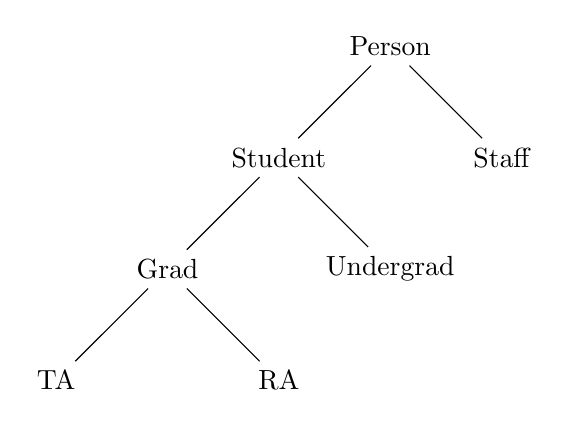
\begin{tikzpicture}[node distance=2cm]
   \node (0) {Person};
   \node (1) [below left of=0] {Student};
   \node (2) [below left of=1] {Grad};
   \node (3) [below left of=2] {TA};
   \node (4) [below right of=0] {Staff};
   \node (5) [below right of=1] {Undergrad};
   \node (6) [below right of=2] {RA};
   \draw (0) -- (1);
   \draw (0) -- (4);
   \draw (1) -- (2);
   \draw (1) -- (5);
   \draw (2) -- (3);
   \draw (2) -- (6);
  \end{tikzpicture}
\end{center}
\caption{A Subtype Hierarchy}
\end{figure}
%\begin{center}
%\begin{picture}(0,140)(0,-20)
%\put(0,0){\makebox(0,0){RA}}
%\put(-80,0){\makebox(0,0){TA}}
%\put(-40,40){\makebox(0,0){Graduate}}
%\put(40,40){\makebox(0,0){Undergrad}}
%\put(0,80){\makebox(0,0){Student}}
%\put(80,80){\makebox(0,0){Staff}}
%\put(40,120){\makebox(0,0){Person}}
%\multiput(-3,6)(40,40)3{\line(-5,4){35}}
%\multiput(-77,6)(40,40)3{\line(5,4){35}}
%\put(0,-20){\makebox(0,0){Figure 1: A Subtype Hierarchy}}
%\end{picture}
%\end{center}
This is an example of a hierarchy that describes a subtype
relationship between different types. In this case, the types Student
and Staff are both subtypes of Person. Alternatively, one can say that
Person is a _supertype_ of Student and Staff. Similarly, TA is a
subtype of the Student and Person types, and so on. The subtype
relationship is normally a preorder (reflexive and transitive) on
types.

A subtype relationship can also be viewed in terms of subsets. If
$\sigma$ is a subtype of $\tau$, then all elements of type $\sigma$
are automatically elements of type $\tau$.

The $\leq$ symbol is typically used to denote the subtype
relationship. Thus, Staff $\leq$ Person, RA $\leq$ Student,
etc. Sometimes the symbol $\lt:$ is used, but we will stick with
$\leq$.

\section{Basic Subtyping Rules}

Formally, we write $\sigma \leq \tau$ to indicate that $\sigma$ is a
subtype of $\tau$. In denotational semantics, this is equivalent to
saying $\SB{\sigma}\subseteq\SB{\tau}$. The informal interpretation of
this subtype relation is that anything of type $\sigma$ can be used in
a context that expects something of type $\tau$. This is known as the
_subsumption_ rule:
\begin{gather*}
\AxiomC{$\Gamma\vdash e:\sigma$}
\AxiomC{$\sigma\leq\tau$}
\BinaryInfC{$\Gamma\vdash e:\tau$}
\DisplayProof
\end{gather*}
Two further general rules are:
\begin{align*}
&
\AxiomC{$\tau \leq \tau$}
\DisplayProof
&&
\AxiomC{$\sigma \leq \tau$}
\AxiomC{$\tau \leq \rho$}
\BinaryInfC{$\sigma \leq \rho$}
\DisplayProof
\end{align*}
which say that $\leq$ is reflexive and transitive, respectively, thus a preorder. In many cases, antisymmetry holds as well, making the subtyping relation a partial order, but this is not always true.

The subtyping rules governing the types 1 and 0 are interesting:
\begin{itemize}
\item 1 ("unit"): Every type is a subtype of 1, that is, $\tau\leq 1$ for all types $\tau$, thus 1 is the top type. If a context expects something of type 1, then it can accept any type. In Java, this is equivalent to the type Object.
\item 0 ("void"): Every type is a supertype of 0, i.e., $0 \leq \tau$ for all types $\tau$, thus 0 is the bottom type. The type 0 can be accepted by any context in lieu of any other type. In Java, this is the type of "null".
\end{itemize}

\subsection{Products and Sums}

The subtyping rules for product and sum types are quite intuitive:
\begin{align*}
&
\AxiomC{$\sigma \leq \sigma'$}
\AxiomC{$\tau \leq \tau'$}
\BinaryInfC{$\sigma * \tau \leq \sigma' * \tau'$}
\DisplayProof
&&
\AxiomC{$\sigma \leq \sigma'$}
\AxiomC{$\tau \leq \tau'$}
\BinaryInfC{$\sigma + \tau \leq \sigma' + \tau'$}
\DisplayProof
\end{align*}
These rules say that the product and sum type constructors are monotone with respect to the subtype relation.
When the subtyping relationship goes in the same direction in the premise as
in the conclusion, it is called a _covariant_ subtyping relationship.

\subsection{Records}

Recall our extensions to the grammar of $e$ and $\tau$ for adding support for record types:
%
\begin{align*}
e\ &::=\ \cdots \bnf \{\ell_1 = e_1, \ldots, \ell_n = e_n\} \bnf e.x\\
\tau\ &::=\ \cdots \bnf \{\type{\ell_1}{\tau_1}, \ldots, \type{\ell_n}{\tau_n}\}
\end{align*}
%
where $n\geq 1$. The $\ell_i$ are called \emph{field identifiers} and are
assumed to be distinct. Also, the order in which they are listed in $\{\ell_1
= e_1, \ldots, \ell_n = e_n\}$ and $\{\type{\ell_1}{\tau_1}, \ldots,
\type{\ell_n}{\tau_n}\}$ does not matter. We also had the following rule added to the small-step semantics:
%
\begin{align*}
\{\ell_1=v_1, \ldots, \ell_n=v_n\}.\ell_i\ &\to\ v_i
\end{align*}
%
as well as the following typing rules:
%
\begin{align*}
&
\AxiomC{$\Gjudge{e_i}{\tau_i},\ 1\leq i\leq n$}
\UnaryInfC{$\Gjudge{\{\ell_1=e_1, \ldots,
\ell_n=e_n\}}{\{\type{\ell_1}{\tau_1}, \ldots, \type{\ell_n}{\tau_n}\}}$}
\DisplayProof
&&
\AxiomC{$\Gjudge e{\{\ldots,x:\tau,\ldots\}}$}
\UnaryInfC{$\Gjudge{e.x}{\tau}$}
\DisplayProof
\end{align*}

There are two subtyping rules for records:
\begin{itemize}
\item _Depth subtyping_: this defines the subtyping relation between two records that have the same number of fields.
\begin{align*}
\AxiomC{$\sigma_i \leq \tau_i,\ 1\leq i\leq n$}
\UnaryInfC{$\{\ell_1:\sigma_1, \ldots, \ell_n:\sigma_n\} \leq
\{\type{\ell_1}{\tau_1}, \ldots, \type{\ell_n}{\tau_n}\}$}
\DisplayProof
\end{align*}
\item _Width subtyping_: this defines the subtyping relation between two records that have different number of fields.
\begin{align}
\AxiomC{$m \leq n$}
\UnaryInfC{$\{\ell_1:\tau_1, \ldots, \ell_n:\tau_n\} \leq
\{\type{\ell_1}{\tau_1}, \ldots, \type{\ell_m}{\tau_m}\}$}
\DisplayProof
\label{eq:depthwidth0}
\end{align}
where the $\leq$ in the premise is integer comparison. Observe that in this case, the subtype has more components than the supertype. This is analogous to the relationship between a subclass and a superclass in which the subclass has all the components of the superclass, which it inherits from the superclass, but perhaps has some components that the superclass does not have.
\end{itemize}

The depth and width subtyping rules for records can be combined into a single rule:
\begin{align}
\AxiomC{$m \leq n\qquad\sigma_i \leq \tau_i,\ 1\leq i\leq m$}
\UnaryInfC{$\{\type{\ell_1}{\sigma_1}, \ldots, \type{\ell_n}{\sigma_n}\} \leq
\{\type{\ell_1}{\tau_1}, \ldots, \type{\ell_m}{\tau_m}\}$}
\DisplayProof
\label{eq:depthwidth}
\end{align}

Mathematically, record types can be viewed as product types whose components
are indexed by the field labels $\ell$. The operators $.\ell$ are the
corresponding projections. Thus if $\Delta$ is a partial function with finite
domain $\dom\Delta$ associating a type $\Delta(\ell)$ with each element $\ell$ in its domain, we might write
\begin{align*}
\prod_{\ell\in\mathsf{dom}\,\Delta} \Delta(\ell)
\end{align*}
for the record type, or just $\prod\Delta$ for short.
An expression of this type would be a tuple indexed by $\dom\Delta$:
\begin{align*}
(e_\ell \mid \ell\in\dom\Delta).
\end{align*}
In this view, the typing rules would take the form
\begin{align*}
&
\AxiomC{$\Gjudge{e_\ell}{\Delta(\ell)},\ \ell\in\dom\Delta$}
\UnaryInfC{$\Gjudge{(e_\ell \mid \ell\in\dom\Delta)}{\prod\Delta}$}
\DisplayProof
&&
\AxiomC{$\Gjudge{e}{\prod\Delta}$}
\UnaryInfC{$\Gjudge{e.\ell}{\Delta(\ell)}$}
\DisplayProof
\end{align*}
and the subtyping rule \eqref{eq:depthwidth} would take the form
\begin{align*}
\AxiomC{$\dom\Delta_1\subseteq\dom\Delta_2$}
\AxiomC{$\Delta_2(\ell)\leq\Delta_1(\ell),\ \ell\in\dom\Delta_1$}
\BinaryInfC{$\prod\Delta_2\leq\prod\Delta_1$}
\DisplayProof
\end{align*}

\subsection{Variants}

The analogous extension for sum types is known as _variant records_ or just
_variants_. These are $\Delta$-indexed coproducts:
\begin{align*}
\sum_{\ell\in\mathsf{dom}\,\Delta} \Delta(\ell)\ &=\ \sum\Delta.
\end{align*}
In OCaml, one would write
\begin{small}
\begin{alltt}
  type t = I of int | S of string | P of int * string
\end{alltt}
\end{small}
to declare the type of a variant record whose elements consist of the (tagged) union of three sets. Here $\dom\Delta=\{\texttt{I},\texttt{S},\texttt{P}\}$ with $\Delta(\texttt{I})=\texttt{int}$, $\Delta(\texttt{S})=\texttt{string}$, and $\Delta(\texttt{P})=\texttt{int * string}$.

The depth subtyping rule for variants is the same as that for records (replacing the records with variants). However, the width subtyping rule is different: instead of $m\leq n$ in \eqref{eq:depthwidth0} and \eqref{eq:depthwidth}, we should take $n\leq m$. Suppose we used the width subtyping rule \eqref{eq:depthwidth0}, the same form as for records. Intuitively, if $\sigma \leq \tau$, then this implies that anything of type $\sigma$ can be used in a context expecting something of type $\tau$. Suppose we now had a "match" statement that did pattern matching on something of type $\tau$. Our subtyping relation says that we can pass in something of type $\sigma$ to this "match" statement and it will still work. However, since $\tau$ has fewer components than $\sigma$ and the "match" statement was originally written for an object of type $\tau$, there will be values of $\sigma$ for which no corresponding case exists. Thus, for variants, the direction of the $\leq$ symbol in the premise needs to be reversed. In other words, for variants, the subtype should have _fewer_ components than the supertype. This leads to the combined rule
\begin{align*}
\AxiomC{$\dom\Delta_1\subseteq\dom\Delta_2$}
\AxiomC{$\Delta_1(\ell)\leq\Delta_2(\ell),\ \ell\in\dom\Delta_1$}
\BinaryInfC{$\sum\Delta_1\leq\sum\Delta_2$}
\DisplayProof
\end{align*}

\section{Function Subtyping}

Based on the subtyping rules we have encountered so far, our first impulse might be to write down something of the following form to describe the subtyping relation for functions:
\begin{align*}
\AxiomC{$\sigma\leq\sigma'$}
\AxiomC{$\tau\leq\tau'$}
\BinaryInfC{$\sigma\to\tau\leq\sigma'\to\tau'$}
\DisplayProof
\end{align*}
However, this is incorrect. To see why, consider the following code fragment:
\begin{quote}
$\letin{f:\sigma\to\tau}g{}$\\
$\letin{f':\sigma'\to\tau'}{g'}{}$\\
$\letin{t:\sigma'}v{}$\\
$f'(t)$
\end{quote}
Suppose $\sigma\leq\sigma'$ and $\tau\leq\tau'$. By the rule above, we would have $\sigma\to\tau\leq\sigma'\to\tau'$, thus we should be able to substitute $f$ for $f'$ and the resulting program should be type correct, provided the original one was. But it is not: if $\sigma'$ is a strict supertype of $\sigma$ and the value $v$ is of type $\sigma'$ but not of type $\sigma$, then $f$ will crash, since it expects an input of type $\sigma$ and it is not getting one.

Actually, the incorrect typing rule given above was implemented in the language Eiffel, and runtime type checking had to be added later to make the language type safe.

The correct subtyping rule for functions is:
\begin{align*}
\AxiomC{$\sigma'\leq \sigma$}
\AxiomC{$\tau\leq\tau'$}
\BinaryInfC{$\sigma\to\tau\leq\sigma'\to\tau'$}
\DisplayProof
\end{align*}
Note that the ordering on the domain is reversed in the premise. Succinctly stated, a function $f$ of type $\sigma\to\tau$ can safely take any input of any subtype $\sigma'$ of $\sigma$, and produces a value that can be taken to be of any supertype $\tau'$ of $\tau$; thus we are free to regard $f$ as a function of type $\sigma'\to\tau'$.

In all the type constructors we had seen so far, the subtyping relation was preserved. With the function space constructor, however, the subtyping relation on the domain is reversed. We say that the function type constructor $\to$ is _contravariant_ in the domain and _covariant_ in the codomain.

\section{References}

Recall the extensions to the grammar of $e$ and $\tau$ for adding support for references:
\begin{align*}
e\ &::=\ \cdots \bnf "ref"~e \bnf !e \bnf e_1 := e_2\\
\tau\ &::=\ \cdots \bnf \tau~"ref"
\end{align*}
The typing rules are
\begin{align*}
&
\AxiomC{$\judge\Gamma e\tau$}
\UnaryInfC{$\judge\Gamma{"ref"~e}{\tau~"ref"}$}
\DisplayProof
&&
\AxiomC{$\judge\Gamma e{\tau~"ref"}$}
\UnaryInfC{$\judge\Gamma{!e}\tau$}
\DisplayProof
&&
\AxiomC{$\judge\Gamma{e_1}{\tau~"ref"}$}
\AxiomC{$\judge\Gamma{e_2}\tau$}
\BinaryInfC{$\judge\Gamma{e_1:=e_2}1$}
\DisplayProof
\end{align*}
As for subtyping, once again our first impulse might be to write down something like the following:
\begin{align*}
\AxiomC{$\sigma \leq \tau$}
\UnaryInfC{$\sigma~"ref" \leq \tau~"ref"$}
\DisplayProof
\end{align*}
However, again this would be incorrect. The problem is that to be safe, a "ref" appearing on the left-hand side of an assignment operator should be contravariant. Consider the following example:
\begin{quote}
$\letin{x:\mathit{Square}~"ref"}{"ref"~\mathit{square}}{}$\\
$\letin{y:\mathit{Shape}~"ref"}x{}$\\
$(\comp{y:=\mathit{circle}}{(!x).\mathit{side}})$
\end{quote}
Even though this code type-checks with the given subtyping rule for reference types, it is not type-correct, since in the last line $x$ does not refer to a square anymore. This problem actually exists in Java when using arrays, as the designers incorrectly used the rule given above. Consequently, a runtime check is necessary.
\begin{alltt}
  public class Test \{
    public static void main(String[] args) \{
      B[] b = new B[1];
      A[] a = b;
      a[0] = new A();
    \}
  \}

  class A \{\}
  class B extends A \{\}

  Exception in thread ``main'' java.lang.ArrayStoreException: A
    at Test.main(Test.java:5)
\end{alltt}
In order to overcome this problem we must use the correct rule below:
\begin{align*}
\AxiomC{$\sigma \leq \tau$}
\AxiomC{$\tau \leq \sigma$}
\BinaryInfC{$\sigma~"ref" \leq \tau~"ref"$}
\DisplayProof
\end{align*}
The subtyping rule for references is thus both covariant and contravariant.
